\documentclass[Visionprosjekt.tex]{subfiles}
\NormalTopp
\begin{document}

%%%%%%%%%%%%%%%%%%%%%%%%%%%%%%%%%%%%%%%%%%%%%%%%
\section{Brukergrensesnitt og PLS-program}
%%%%%%%%%%%%%%%%%%%%%%%%%%%%%%%%%%%%%%%%%%%%%%%%

Dette kapitlet beskriver og dokumenterer brukergrensesnittet og PLS-programmet.



%%%%%%%%%%%%%%%%%%%%%%%%%%%%%%%%%
\subsection{Brukergrensesnittet}
%%%%%%%%%%%%%%%%%%%%%%%%%%%%%%%%%
Ved hjelp av WinCC er det laget et brukergrensesnitt som inneholder følgende.

\begin{itemize}
    \item En grafisk representasjon av systemet med  sensorer, stempel og motorer.
	\item Innstillinger for dosering av stoff $A$ og $B$ for de ulike produktene.
    \item Mulighet for å avbryte sekvensen (ved å sette anlegget i manuell modus).
    \item Mulighet for å styre stempel og motorer manuelt.
    \item Visning og logging av alarmer (sikkerhetsstråle brutt eller nødstopp aktivert).
    %\item Visning av informasjon fra frekvensomformer -- data fra feltbussnode.
\end{itemize}



 \refF{fig:auto_kjorer} viser anlegget mens den automatiske fyllesyklusen kjøres.
Endring av motorfrekvensen og oppheving av sikkerhetsmodus, krever passord. Innlogging skjer ved å trykke F10 og fylle ut informasjonen nedenfor.

\begin{center}
    \begin{tabular}{ll}
        Brukernavn: & \texttt{Espen}\\
        Passord: & \texttt{123456}
    \end{tabular}
\end{center}

Innloggingsinformasjonen er også skrevet direkte på skjermbildet. Dette gjøres selvsagt ikke i et reellt brukergrensesnitt i industrien.

%Designet og funksjonene er programmert i henhold til HMI standarddokument.




%Modellen kan kjøres på to måter, manuell  eller automatisk modus.
%
%Ved normal drift vil båndet kjøres i automatisk modus.
%Det er mulig å kjøre transportbåndet manuelt. I denne modusen er lysgardinen koplet ut. Kjøring i manuell modus gjøres normalt ikke. Dersom båndet stopper på grunn av nødstopp må båndet startes opp i manuell modus.
%
%Enkelte valgmuligheter er også passordbeskyttet. Dette gjøres for ar ikke uvedkommende skal gjøre skade på systemet. Funksjoner som er passordbeskyttet er valg av hastighet på båndet og kvittering av alarmer.
%


%\clearpage

\subsubsection{Organisering}

\begin{wrapfigure}{r}{48mm}
	\centering
    \vspace{-10pt}
		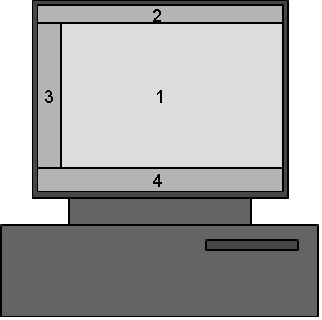
\includegraphics[scale=0.8]{bilder/skjermomraader.pdf}
	\caption{Inndeling av en PC-skjerm }
	\label{fig:skjermomraader}
\end{wrapfigure}
Organisering av elementer på brukergrensesnittets skjermbilde er gjort i tråd med retningslinjer gitt i HiTs standarddokument for HMI, samt generelle tips  \cite{HMIstandard,HMIMorten}. Utgangspunktet for skjermbildet er  \reff{fig:skjermomraader} \cite{HMIstandard}.

%Brukergrensesnittet  er designet etter retningslinjer gitt ved høgskolens HMI-standarddokument samt generelle tips  \cite{HMIstandard,HMIMorten}. Utgangspunktet for skjermbildet har vært  \reff{fig:skjermomraader} \cite{HMIstandard}.

%\begin{figure}[ht]
	%\centering
		%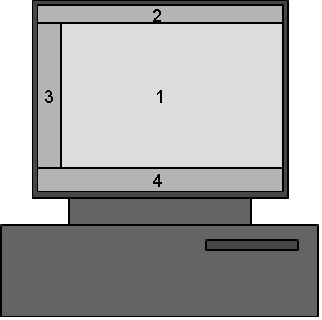
\includegraphics[scale=0.8]{bilder/skjermomraader.pdf}
	%\caption{Inndeling av en PC-skjerm }
	%\label{fig:skjermomraader}
%\end{figure}



I følge standarddokumentet bør områdene 1--4 inneholde følgende elementer.
\begin{enumerate}
	\item Prosessbilde.
    \item Navigering mellom prosessbilder, oversikt over alarmer og navigering til alarmlister.
    \item Navigering mellom prosessbilder.
    \item Funksjoner som ikke er viktig  i forhold til prosessen.
\end{enumerate}



\clearpage
Brukergrensesnittet for anlegget er organisert slik:
\begin{description}[style=multiline,leftmargin=22mm]

    \item[Område 1] I område 1 finnes hoveddelen av brukergrensesnittet. Her finnes oversiktstegning av anlegget med sensorer, motorer og stempel. Funksjoner for valg av fylling og sortering er lagt her, samt alarmlogg. Kontroller for tvangskjøring av stempel og motorer vises  når manuell modus er valgt.

    \item[Område 2] Område 2 brukes til overskrifter og logo. Denne delen brukes kun til opplysning om hvilken anleggsdel brukergrensesnittet gjelder for. I dette tilfellet er det tilstrekkelig med ett skjermbilde.

    \item[Område 3] Til venstre i skjermbildet, er navigasjonsknapper for valg av manuell eller automatisk modus plassert.

    \item[Område 4]  I bunnen av bildet finnes klokke, knapp for å avslutte brukergrensesnittet (WinCC) og innloggingsinformasjon.

\end{description}




\begin{figure}[ht]
	\centering
		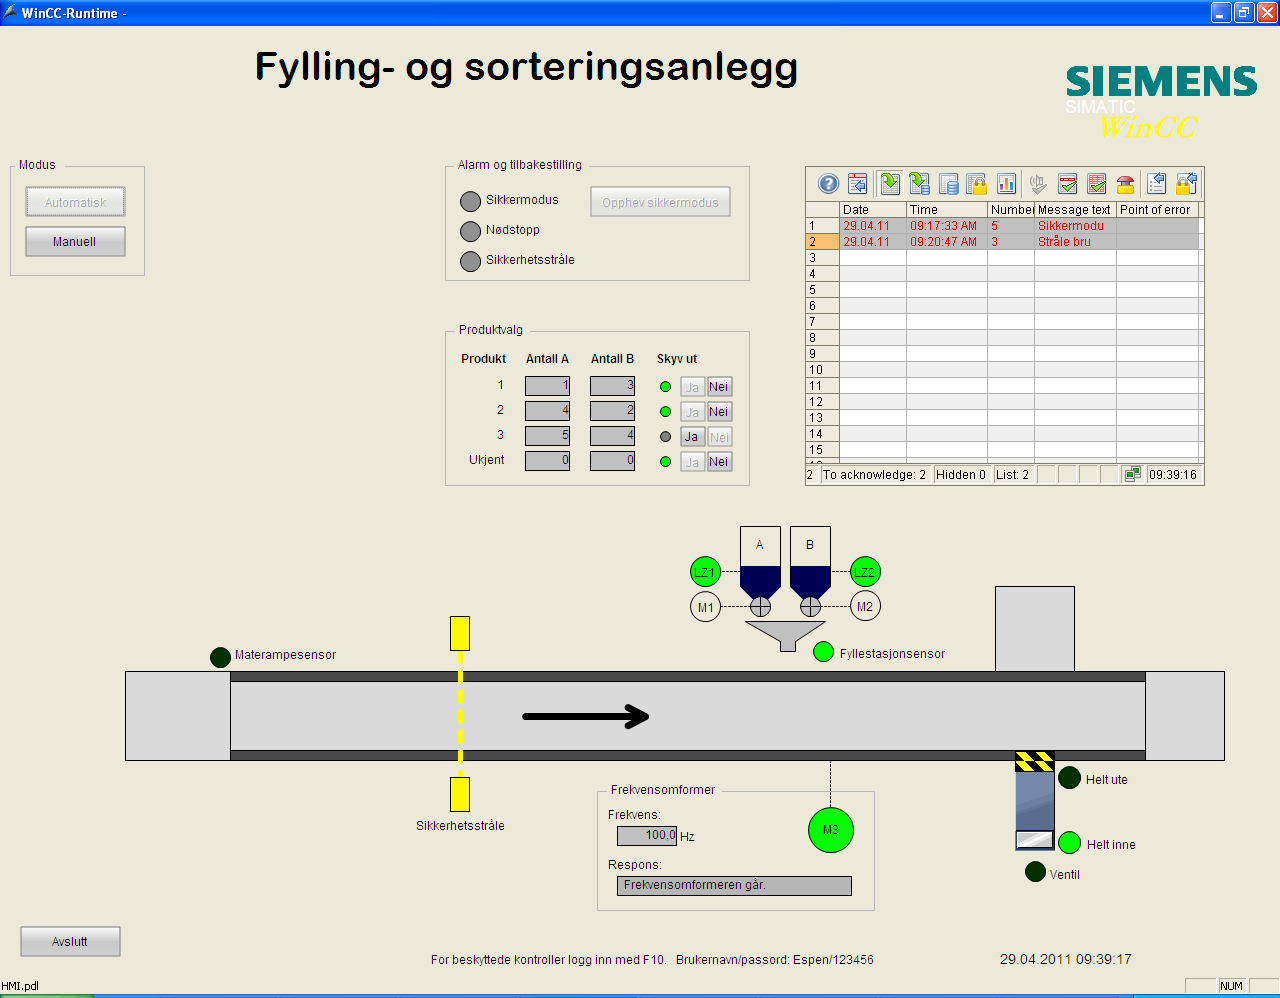
\includegraphics[width=1.0\textwidth]{bilder/auto_kjorer}
	\caption{HMI, automatisk modus}
	\label{fig:auto_kjorer}
\end{figure}






\subsubsection{Fargevalg}

Ved utforming av et brukergrensesnitt er fargevalg viktig \cite{HMIstandard}.
Det lagt vekt på bruk av kontraster, for å tiltekke oppmerksomhet og gjøre skjermbildet behagelig å se på. Fargene er få og  ensbetydende, slik at feiltolkning skal unngås. Fargen rød er f.eks kun brukt til alarmer og alarmkilder.
Et eksempel på fargebruk ved alarm er vist på \reff{fig:strale_brutt}. Her går det klart og tydelig frem at sikkerhetsstrålen er brutt, og at anlegget har gått i sikkerhetsmodus.


\begin{figure}[ht]
	\centering
		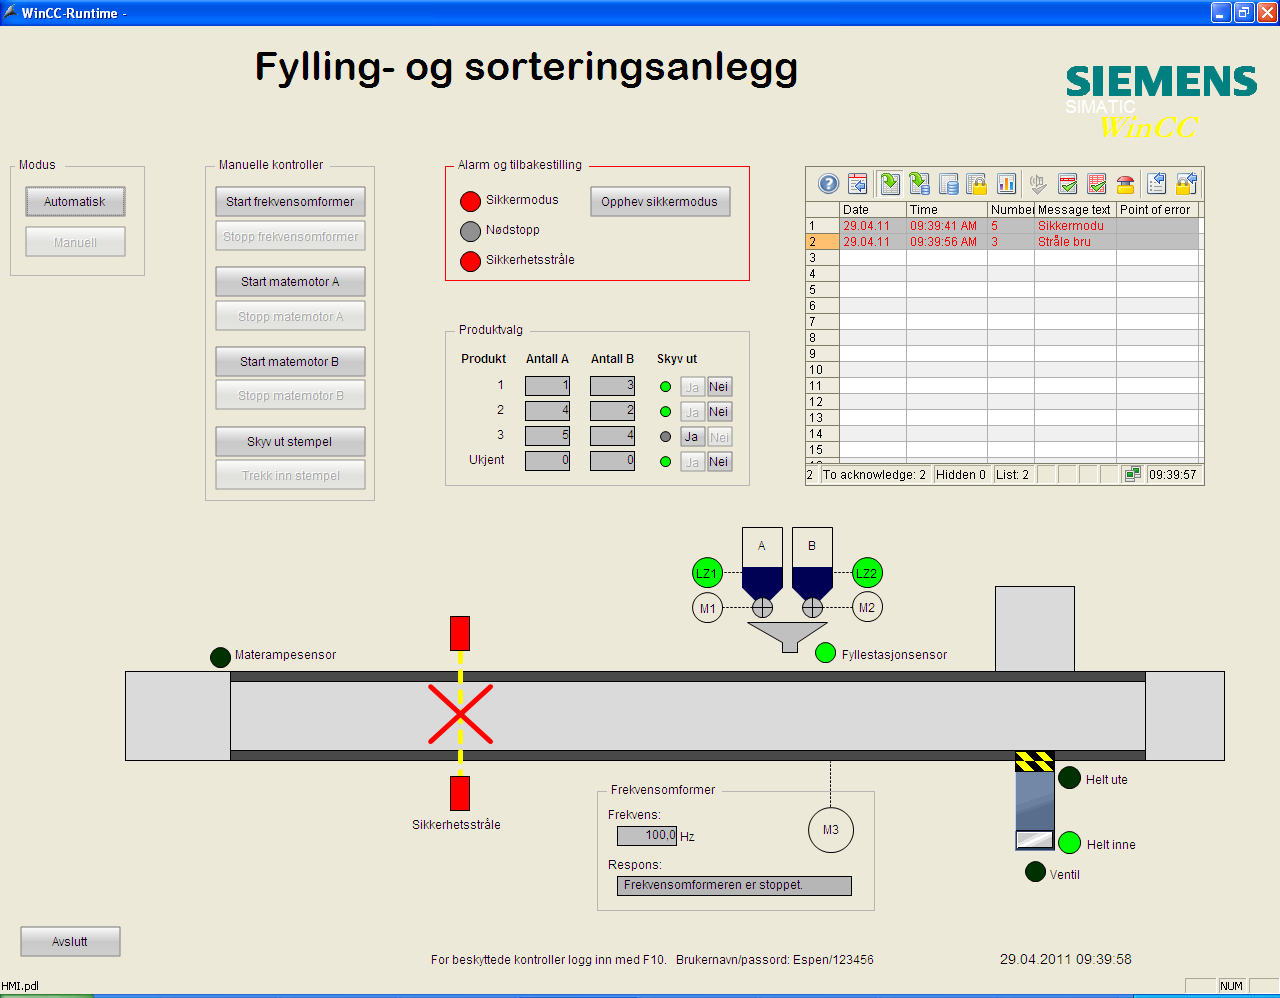
\includegraphics[width=1.0\textwidth]{bilder/strale_brutt}
	\caption{HMI, manuell modus med sikkerhetsstråle brutt}
	\label{fig:strale_brutt}
\end{figure}





\subsubsection{Produktvalg}

Vision-kameraet er satt opp til å gjenkjenne tre ulike «produkter». Et «produkt» i denne sammenhengen er definert som  en blanding av en gitt mengde  av stoff $A$ og en gitt mengde av $B$. En binærverdi  bestemmer om beholderen med produktet skal skyves ut av stempelet. \refF{fig:produktvalg} er et utsnitt av brukergrensesnittet, som viser hvordan operatøren kan styre oppsettet av  produktene. Fyllingsgradene til bokser/datamatriser som ikke er gjenkjent kan også stilles inn, selv om de i de fleste tilfeller vil være som på figuren; ingen fylling og utskyvning aktivert.

\begin{figure}[ht]
	\centering
		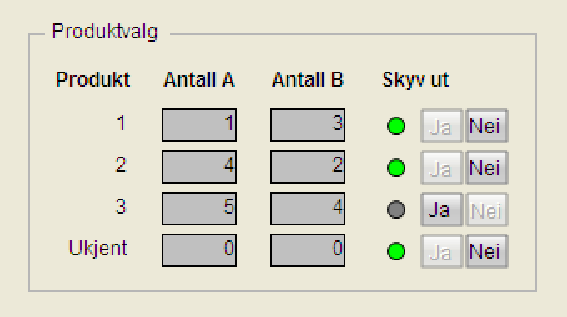
\includegraphics[scale=0.8]{bilder/produktvalg.pdf}
	\caption{Utsnitt av brukergrensesnittet som viser produktvalg}
	\label{fig:produktvalg}
\end{figure}



\subsubsection{Vurdering av HMI standarddokument}
\label{subsec:HMI-vurdering}

Høgskolens standarddokument for HMI-design er brukt som retningslinjer ved utvikling av brukergrensesnittet til transportbåndmodellen.
Imidlertid viste det seg  at dokumentet ikke var fullgodt. På noen områder er det derfor brukt skjønn ved utforming av brukergrensenittet.


%Det ble derfor brukt skjønn i de tilfeller der dokumentet sviktet, for å utvikle et design for best mulig brukervennlighet.


%Høgskolens standarddokument \cite{HMIstandard} bør utvides og konkretiseres. En forbedring vil være å spesifisere fargekoder (f.eks. RGB eller HTML-format) for de ulike tilstandene og elementene, ikke bare fargenavnet.
Høgskolens standarddokument har klare mangler og bør utvides og konkretiseres.
Prosjektet har resultert i følgende liste over nødvendige forbedringer.


\begin{itemize}
	\item Fargekoder spesifiseres (f.eks. i RGB- eller HTML-format) for de ulike tilstandene og elementene, ikke bare fargenavnet.
    \item Skjermoppløsning  bør omtales.
    \item Størrelse på skrift spesifiseres i forhold til skjermoppløsning og font.
    \item Plassering og justering av tekst og tall i tekstbokser må spesifiseres. Tall skal alltid høyrejusteres.
    \item Antall desimaler og desimalskilletegn i numeriske verdier bør omtales.
    \item Størrelser på de vanligste enhetene i et P\&ID-diagram bør defineres.
    \item Et konkret eksempel på et fullstendig brukergrensesnitt bør være med, gjerne to -- et stort og et lite anlegg. «Et bilde sier mer enn 1000 ord.»
    \item Det bør forklares hvordan navigering i skjermbildet vha. tabulator-tasten skal foregå.
\end{itemize}




%%%%%%%%%%%%%%%%%%%%%%%%%%%%%%%%
\subsection{PLS-programmet}
%%%%%%%%%%%%%%%%%%%%%%%%%%%%%%%%


Det er benyttet både FBD og SFC til programmeringen. Programmet er oppdelt i programblokker av hensyn til ryddighet. Blokkene tar seg av ulike oppgaver, beskrevet nedenfor. %Parentesen angir programmeringsspråket som er benyttet for blokken.


\begin{description}[style=multiline,leftmargin=13mm]

    \item[OB1] Dette er PLS-programmets hovedblokk, hvor de andre blokkene blir kalt opp. Overordnet styringslogikk for aktivering og deaktivering av blokker er også inkludert her. Blokken er programmert i FBD. \refV{ved:ob1} viser programkoden for OB1.

    % i riktig rekkefølge.

    \item[FB1] Her ligger sekvensdiagrammet som styrer anlegget i automatisk modus. Dette er nærmere beskrevet i systembeskrivelsen, kapittel \ref{subsec:auto}. Blokken er laget i SFC,  som gir en god oversikt over programflyten og -strukturen. Noen av overgangsbetingelsene er laget vha. FBD i FC1. \refV{ved:sfc} viser programkoden for FB1.


    %Noen overgangsbetingelser som krever FBD, er laget i FC1.

    \item[FB2] Tar seg av kommunikasjon med frekvensomformeren. FBD er benyttet til programmeringen. Denne blokken er basert på profibus-adapterens manual \cite{profibusadapter}. \refV{ved:frekvensomformerprogram} viser programkoden for FB2.

    \item[FC1] Denne blokken inneholder en del hjelpefunksjoner, i tillegg til logikken rundt  sikkerhetsmodus, tolking av kamerasignal og manuell modus. Overgangsbetingelser i sekvensprogrammet FB1 som krever FBD, er også programmert her. \refV{ved:hjelp} viser programkoden for FC1.

\end{description}



%
%\begin{table}[ht]%
    %\centering
    %\caption{Programblokker}
    %\renewcommand\arraystretch{1.2}
    %%\small
    %\begin{tabularx}{\textwidth}{ll>{\raggedright\arraybackslash}l>{\raggedright\arraybackslash}X}
        %\toprule
        %Navn	&  Språk & Dokumentasjon & Beskrivelse  \\
        %\midrule
        %OB1   &  FBD  & \refV{ved:ob1}   & Hovedblokk som kaller opp de andre blokkene. \\
        %FB1   &  SFC  & \refV{ved:sfc}   & Sekvensdiagrammet som styrer anlegget i automatisk modus, beskrevet i systembeskrivelsen, kapittel \ref{subsec:auto}. \\
        %FC1   &  FBD  & \refV{ved:hjelp} & Styrer logikken rundt  sikkerhetsmodus, tolking av kamerasignal og manuell modus.\\
        %FB2   &  FBD  & \refV{ved:frekvensomformerprogram}  & Tar seg av kommunikasjon med frekvensomformeren, er laget ut ifra profibusadapterets manual \cite{profibusadapter}. \\
        %\bottomrule
	%\end{tabularx}
    %\label{tab:blokker}
%\end{table}



PLS-programmet er satt opp etter tilordningslisten i \reft{tab:tilordning}. De neste underkapitlene vil ta for seg sikkerhetsfunksjoner og styring av frekvensomformeren.

\begin{table}[ht]
\footnotesize    \renewcommand\arraystretch{1.2}
    \centering
    \caption{Tilordningsliste for PLS}
    \label{tab:tilordning}
    %\begin{tabularx}{1.0\textwidth}{>{\ttfamily}lrlX}
    \begin{tabular}{>{\ttfamily}lrll}
            \toprule   
        \multicolumn{4}{c}{Utgangsmodul PLS2}\\ 
            \midrule
            \normalfont Utg.  &  Skrue  & Ref. &  Beskrivelse	\\ 
            \midrule 
            Q0.0  &  2  &  SB1  & Resett SafeBox (dobbel kortvarig impuls)	\\ 
            Q0.1  &  3  &  K1  & Start relé 1 -- skruemotor fyllstoff A	\\ 
            Q0.2  &  4  &  K2  & Start relé 2 -- skruemotor fyllstoff B	\\ 
            Q0.3  &  5  &  MV1 & Skyv ut stempel (går automatisk tilbake når spenning forsvinner)	\\
            %Q0.4  &  6  &	\\
            %Q0.5  &  7  &	\\
            %Q0.6  &  8  &	\\
            %Q0.7  &  9  &	\\
							\\
			Q1.0  &  12  &  DVB1   & Trigg kamera (ta bilde)	\\ 
            %Q1.1  &  13  &  \\
            %Q1.2  &  14  &  \\
            %Q1.3  &  15  & 	\\
            %Q1.4  &  16  & 	\\
            %Q1.5  &  17  & 	\\
            %Q1.6  &  18  & 	\\
            %Q1.7  &  19  & 	\\
            \midrule
        \multicolumn{4}{c}{Inngangsmodul PLS4}\\ 
            \midrule
            \normalfont Inng.  &  Skrue  & Ref. &   Beskrivelse\\ 
            \midrule
            I0.0  &  2  &  LZ7 & Sensor ved materampe			\\  	 
            I0.1  &  3  &  FC2 & Sensor ved kamera				\\  	 
            I0.2  &  4  &  FC3 & Sensor ved fyllestasjon		\\  	 
            I0.3  &  5  &  LZ1 & Tomt for stoff A (invertert)	\\ 
            I0.4  &  6  &  LZ2 & Tomt for stoff B (invertert)	\\ 
            I0.5  &  7  &  LZ3 & Bulkteller stoff A (impuls)	\\ 
            I0.6  &  8  &  LZ4 & Bulkteller stoff B (impuls)	\\ 
            I0.7  &  9  &  LZ5 & Stempel helt ute				\\ 
            \\ 
            I1.0  &  12  & LZ6 & Stempel inne -- normalposisjon \\ 
            I1.1  &  13  & SB1  & SafeBox har gått i sikkerhetsmodus pga. lysgitter (invertert) 	 \\ 
            I1.2  &  14  & SB1  & SafeBox har gått i sikkerhetsmodus pga. nødstopp (invertert) 	 \\ 
            %I1.3  &  15  &	\\ 
            %I1.4  &  16  &	\\ 
            %I1.5  &  17  &	\\ 
            %I1.6  &  18  & 	\\ 
            %I1.7  &  19  & 	\\ 
            \\ 
            I2.0  &  22  & DVB1 & Digital utgang fra kamera -- produkt 1	\\ 
            I2.1  &  23  & DVB1 & Digital utgang fra kamera -- produkt 2	\\ 
            I2.2  &  24  & DVB1 & Digital utgang fra kamera --  produkt 3	\\ 
            I2.3  &  25  & DVB1 & Digital utgang fra kamera  			\\ 
            I2.4  &  26  & DVB1 & Digital utgang fra kamera 	 			\\ 
            I2.5  &  27  & DVB1 & Digital utgang fra kamera 				\\ 
            I2.6  &  28  & DVB1 & Digital utgang fra kamera -- opptatt				\\ 
            \\ 
        \bottomrule
    %\end{tabularx}
    \end{tabular}
\end{table}





\clearpage
\subsubsection{Sikkerhet}

Dersom nødstoppbryteren aktiveres eller sikkerhetsstrålen blir brutt, vil sikkerhetsmonitoren og PLS-programmet gå over i sikkermodus. Sikkerhetsmonitoren vil stoppe alle bevegelige deler momentant, uten å gå via PLS-en. Samtidig vil PLS-programmet resette sekvensen, stoppe alle bevegelige deler (programvaremessig) og gå over i manuell modus. For å oppheve sikkerhetsmodusen må

\begin{enumerate}
    \item årsaken til feilen fjernes (blokkering av lysgardin/nedtrykt nødstopp) og
	\item en bekreftelse gis fra brukergrensesnittet (passordbeskyttet).
\end{enumerate}



\subsubsection{Styring av frekvensomformer}

For å  starte frekvensomformeren må det overføres et kontrollord fra PLS-en til frekvensomformerens dataadresse i profibus-nettverket. Et "<ord"> eller  \texttt{WORD}  i denne sammenheng, er en 16-bits heksadesimal kode. I tillegg må det overføres et referanseord med verdi i området $\pm 20\,000$. Referanseordet  bestemmer frekvensen, og blir skalert om til $\pm\text{maks}$\-imal frekvens. Maksimal frekvens velges i frekvensomformerens innstillinger i parameter \texttt{1105 EXT REF1 MAX}.

\textit{Eksempel:}\\
%\hfil \begin{parbox}[r]{0.8\textwidth}
%\parbox{0.8\textwidth}{
\hangindent=6mm
Maksimalfrekvensen $f_\text{max}= 100$\,Hz er satt i parameter \texttt{1105 EXT REF1 MAX}.
Referanseordet 10\,000 blir overført til frekvensomformeren fra PLS-programmet.  Frekvensen ut til motoren blir $f_\text{ut}=50$\,Hz, beregnet i \reffo{equ:frekv}. \cite{profibusadapter}

\begin{equation}
    f_\text{ut}=
    \frac{\text{Referanseord} \cdot f_\text{max}}{20\,000}=
    \frac{10\,000  \cdot  100\,\text{Hz}}{20\,000} = 50\,\text{Hz}
    \label{equ:frekv}
\end{equation}

%\end{parbox}
%}



\blanklines{1}
Frekvensomformeren kan innta forskjellige tilstander, f.eks.:
\begin{itemize}
     \item Klar/ ikke klar til å starte.
     \item Oppramping (frekvensen øker som en del av oppstarten).
     \item Kjører.
     \item Nødstopptilstand.
     \item Feiltilstand.
\end{itemize}
 Noen av  tilstandene krever at spesifikke kontrollord blir overført før frekvensomformeren kan startes, f.eks. nødstopptilstanden. Hvilken tilstand som er aktiv, leses i et statusord som overføres  til PLS-en. \cite{profibusadapter}

Det er laget en funksjonsblokk i PLS-programmet (FB2) for korrekt styring av frekvensomformeren. Funksjonsblokkens inn- og utganger er listet  opp i \reft{tab:frekvblokk}.


%innganger for start (\texttt{BIT}), stopp (\texttt{BIT}) og hastighet (\texttt{FLOAT}), i tillegg til utganger for avlesning av aktuell hastighet (\texttt{FLOAT}) og om motoren kjører (\texttt{BIT}).

 Hjelpefunksjonene FC104 og FC105 sørger for riktig skalering av hastighet. %\refF{fig:frekvensblokk} viser funksjonsblokken.
Se \refv{ved:frekvensomformerprogram} for programkoden.




\begin{table}[ht]%
    \centering
    \caption{Frekvensomformerblokkens inn- og utganger}
    \renewcommand\arraystretch{1.2}
    %\small
    \begin{tabular}{ll>{\ttfamily}l>{\raggedright\arraybackslash}l}
        \toprule
        Funksjon	        &  Retning & \normalfont Datatype   \\
        \midrule
        Start               &  Inngang  & BIT   \\
        Stopp               &  Inngang  & BIT     \\
        Hastighet           &  Utgang   & FLOAT   \\
        Aktuell hastighet   &  Utgang   & FLOAT   \\
        \bottomrule
	\end{tabular}
    \label{tab:frekvblokk}
\end{table}














%\begin{figure}[ht]
%\centering
		%
\includegraphics[scale=0.5]{bilder/frekvensblokk.pdf}
	%\caption{Funksjonsblokk for PLS-styring av frekvensomformer}
	%\label{fig:frekvensblokk}
%\end{figure}
%
%


%
%
%\subsubsection{Signaloverføring}
%
%Signalene mellom PLS, ekstern I/O og frekvensomformer går over feltbuss. Det benyttes her Profibus DPti kommunikksjon mellom enhetene. Dette er satt opp i PLS slik (figuren) viser.
%
%I bussnettveket er alle enheter gitt hver sin unike adresse i nettverket. PLS-en er gitt adressen 2 den eksterne I/O modulen er gitt adressen 12 og frekvensomformeren er gitt adressen 8.
%Modellenes digitale sensorer er koplet til I/O-moduler på modellenes koplingsbrett. Fra vision-senseoren sendes 4 digitale signaler til I/O moduler, hvert signal sier hvilket produkt som skal fylles. Via digitale utganger styres tre releer. Et til hever av motorene i fyllestasjonen og et til styring av pneumatikkventilen.


\end{document}